\chapter{System architecture}

The system design described in this chapter is part of the Cerberus visualization framework [Reference?]. First of all the module design of the framework is depicted. This design overview is followed by a rather detailed presentation of selected sub-modules. Finally the mapping process of the gene-expression data onto the metabolic pathways is conceptually outlined.

\section{Overall Design}

Platform independent

\begin{figure}[ht]
\centering
\scalebox{0.4}{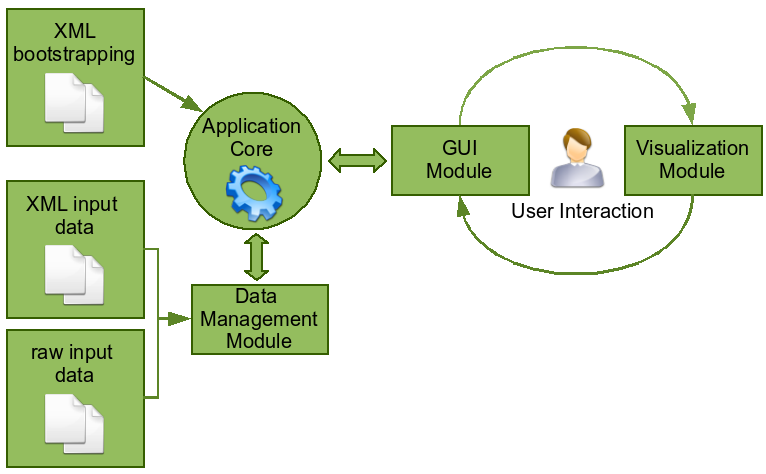
\includegraphics{gfx/application_block_chart}} 
\caption[Application block chart]{\textit{Application block chart}} 
\label{gfx:application_block_chart}
\end{figure}

\section{Pathway Data Management}

From information point of view metablic pathways are graphs. The nodes are enzymes and compounds. The edges can be differenciated in relations and reactions.

\begin{figure}[ht]
  \centering
    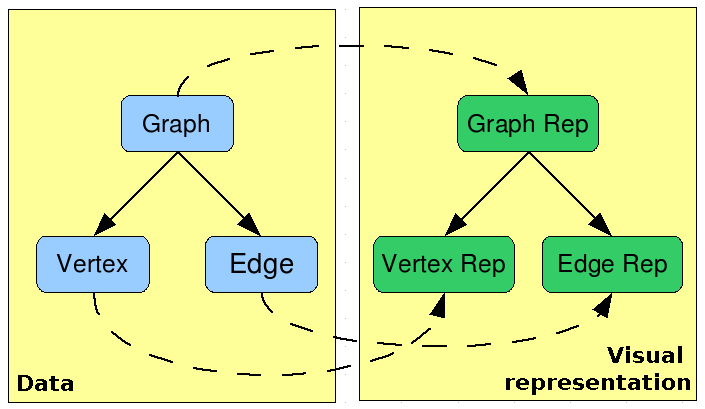
\includegraphics[width=0.5\linewidth]{gfx/model_view_data_diagram}
  \caption{Model abstraction into data and visual representations}
  \label{fig:model_view_data_diagram}
\end{figure}

[The problem description why this solution is needed is very good described in \cite{Bourqui2006}.]

[Describe idea of data proxy]

\begin{figure}[ht]
  \centering
    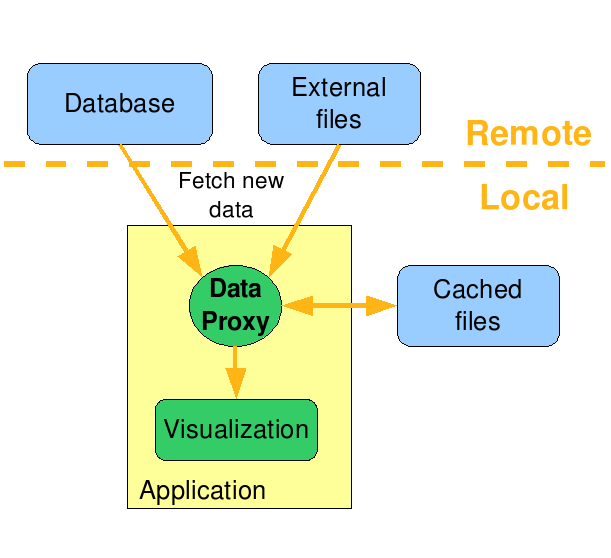
\includegraphics[width=0.5\linewidth]{gfx/data_block_diagram_new}
  \caption{Data block diagram showing the data loading process}
  \label{fig:data_block_diagram}
\end{figure}

[Insert UML diagram of pathway data management]

%\subsection{Set / Storage / Virtual Array}

%Referenz auf Michaels Thesis

\section{Graphical User Interface (GUI)}

Graphical user interface of the Cerberus framework is set up using the SWT library (Referenz!) The system is designed to support fast creation of new visualization setups. Parametrized via XML configuration file arbitrary layouts. Views are positioned arbitrary forming a new setup. A view is a container 

[Insert UML diagram of GUI-Manager \& View-Manager]
[Describe layouting of framework - container can hold several views]

[Define what we mean by a VIEW]

Views:
- 2D Pathway
- 3D Pathway
- Scatterplot
- Heatmap etc.


\section{Data update (notification) mechanism}

A data update is the process of changing data and in turn informing related parties. Objects of the systems are qualified to receive update notifications if they somehow act on this data. The receiver can decide what actions will be triggered.
 
[Insert UML diagram]

%Selection handling included 

\section{Enzyme-Gene Mapping}

For realizing the mapping of enzymes onto the pathway we had to face the question how to store the data. Considering the fact that the framework has to handle several thousands of enzymes and up to the factor of 10 more genes the design descision needed to be well considered. The complete mapping tables are loaded into RAM at startup and are held during runtime. Of course, this approach increases the working memory consumption of our application considerable. However, the considerably high working memory consumption is consciously accepted because the requirements focuses cleary onb short mapping times.

For each external identification number (e.g. enzyme codes, gene accessions, etc.) that is fed into the system an internal ID is generated. The idea behind that procedure is that in every stage of the system the type of data can be fastly determined by investigating the ID. The disadvantage that this approach brings along is that an external to internal ID mapping table needs to be accessible at any time. 

The mapping mechanism must take care of the fact that a bidirectional conversion of most ID types is required.\\
Example: User selects an enzyme inside a pathway and want to know which genes produce that particular protein (i.e. mapping from enzymes to genes). On the other hand in for example a scatterplot that visualizes gene-expression results the user might be interested in the encoding of which enzymes a particular gene is involved (mapping from genes to enzymes).

\begin{figure}[ht]
\centering
\scalebox{0.45}{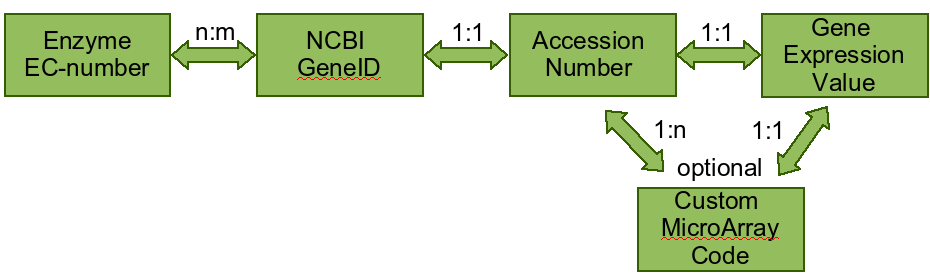
\includegraphics{gfx/enzyme_gene_mapping}} 
\caption[Enzyme-Gene Mapping]{\textit{Enzyme-Gene Mapping}} 
\label{gfx:enzyme_gene_mapping}
\end{figure}

Our framework is capable of visualizing different gene mapping methods:
\begin{itemize}
 \item Multiple gene mapping
 \item Time series gene-expression visualization
\end{itemize} 

Map at end of pipeline points to storage (by holding the index as value)\\
GenomeId manager configuration via XML file\\

[Decide where to put the text]
When multiple views are connected and the sent data needs to be mapped this procedure takes place inside the update callback method of the receiver. This policy origins in the consideration that only the target view knows how to map the data because that is the point where the information is going to be visualized. This is also the perfect place for filtering the data (e.g. ignore data that is useless for the visualization in that view).